%%%%%%%%%%%%%%%%%%%%%%%%%%%%%%%%%%%%%%%%%
% University/School Laboratory Report
% LaTeX Template
% Version 3.0 (4/2/13)
%
% This template has been downloaded from:
% http://www.LaTeXTemplates.com
%
% Original author:
% Linux and Unix Users Group at Virginia Tech Wiki
% (https://vtluug.org/wiki/Example_LaTeX_chem_lab_report)
%
% License:
% CC BY-NC-SA 3.0 (http://creativecommons.org/licenses/by-nc-sa/3.0/)
%
%%%%%%%%%%%%%%%%%%%%%%%%%%%%%%%%%%%%%%%%%

%----------------------------------------------------------------------------------------
%	PACKAGES AND DOCUMENT CONFIGURATIONS
%----------------------------------------------------------------------------------------

\documentclass{article}

\usepackage{mhchem} % Package for chemical equation typesetting
\usepackage{siunitx} % Provides the \SI{}{} command for typesetting SI units
\usepackage{hyperref}
\usepackage{graphicx} % Required for the inclusion of images
\usepackage{tabularx}
\usepackage{float}
\usepackage{algorithm}
\usepackage{algpseudocode}
\usepackage{bm}
\usepackage{multirow}% http://ctan.org/pkg/multirow
\usepackage{hhline}% http://ctan.org/pkg/hhline
\usepackage{caption}
\usepackage{subcaption}
\usepackage{listings}
\usepackage{xcolor}
\usepackage[letterpaper, margin=0.9in]{geometry}
\lstset{
    %numbers=left,
    stepnumber=1,    
    firstnumber=1,
    numberfirstline=true,
    basicstyle=\ttfamily,
    keywordstyle=\color{blue}\ttfamily,
    stringstyle=\color{red}\ttfamily,
    commentstyle=\color{green}\ttfamily,
    breaklines=true,
}


\setlength\parindent{0pt} % Removes all indentation from paragraphs

\renewcommand{\labelenumi}{\alph{enumi}.} % Make numbering in the enumerate
% environment by letter rather than number (e.g. section 6)

%\usepackage{times} % Uncomment to use the Times New Roman font

%----------------------------------------------------------------------------------------
%	DOCUMENT INFORMATION
%----------------------------------------------------------------------------------------

\title{UC Davis STA 208 2016 Spring Midterm Exam} %
% Title
\author{Wenhao \textsc{Wu}, 998587583} % Author name
\date{\today} % Date for the report

\begin{document}
\maketitle % Insert the title, author and date

% If you wish to include an abstract, uncomment the lines below

\section{Data Description}
This dataset contains $N=3089$ observations of $p=4$ features. Among this
observations $N_0=1089$ observations are labeled with the response $y=0$ and
$N_1= 2000$ observations with $y=1$, and the formers are located in the second
half of the data file while the latter in the first half.
The scatterplot matrix of the dataset is shown in Fig.~\ref{fig:scatterplot}
\begin{figure}[h]
  \centering
  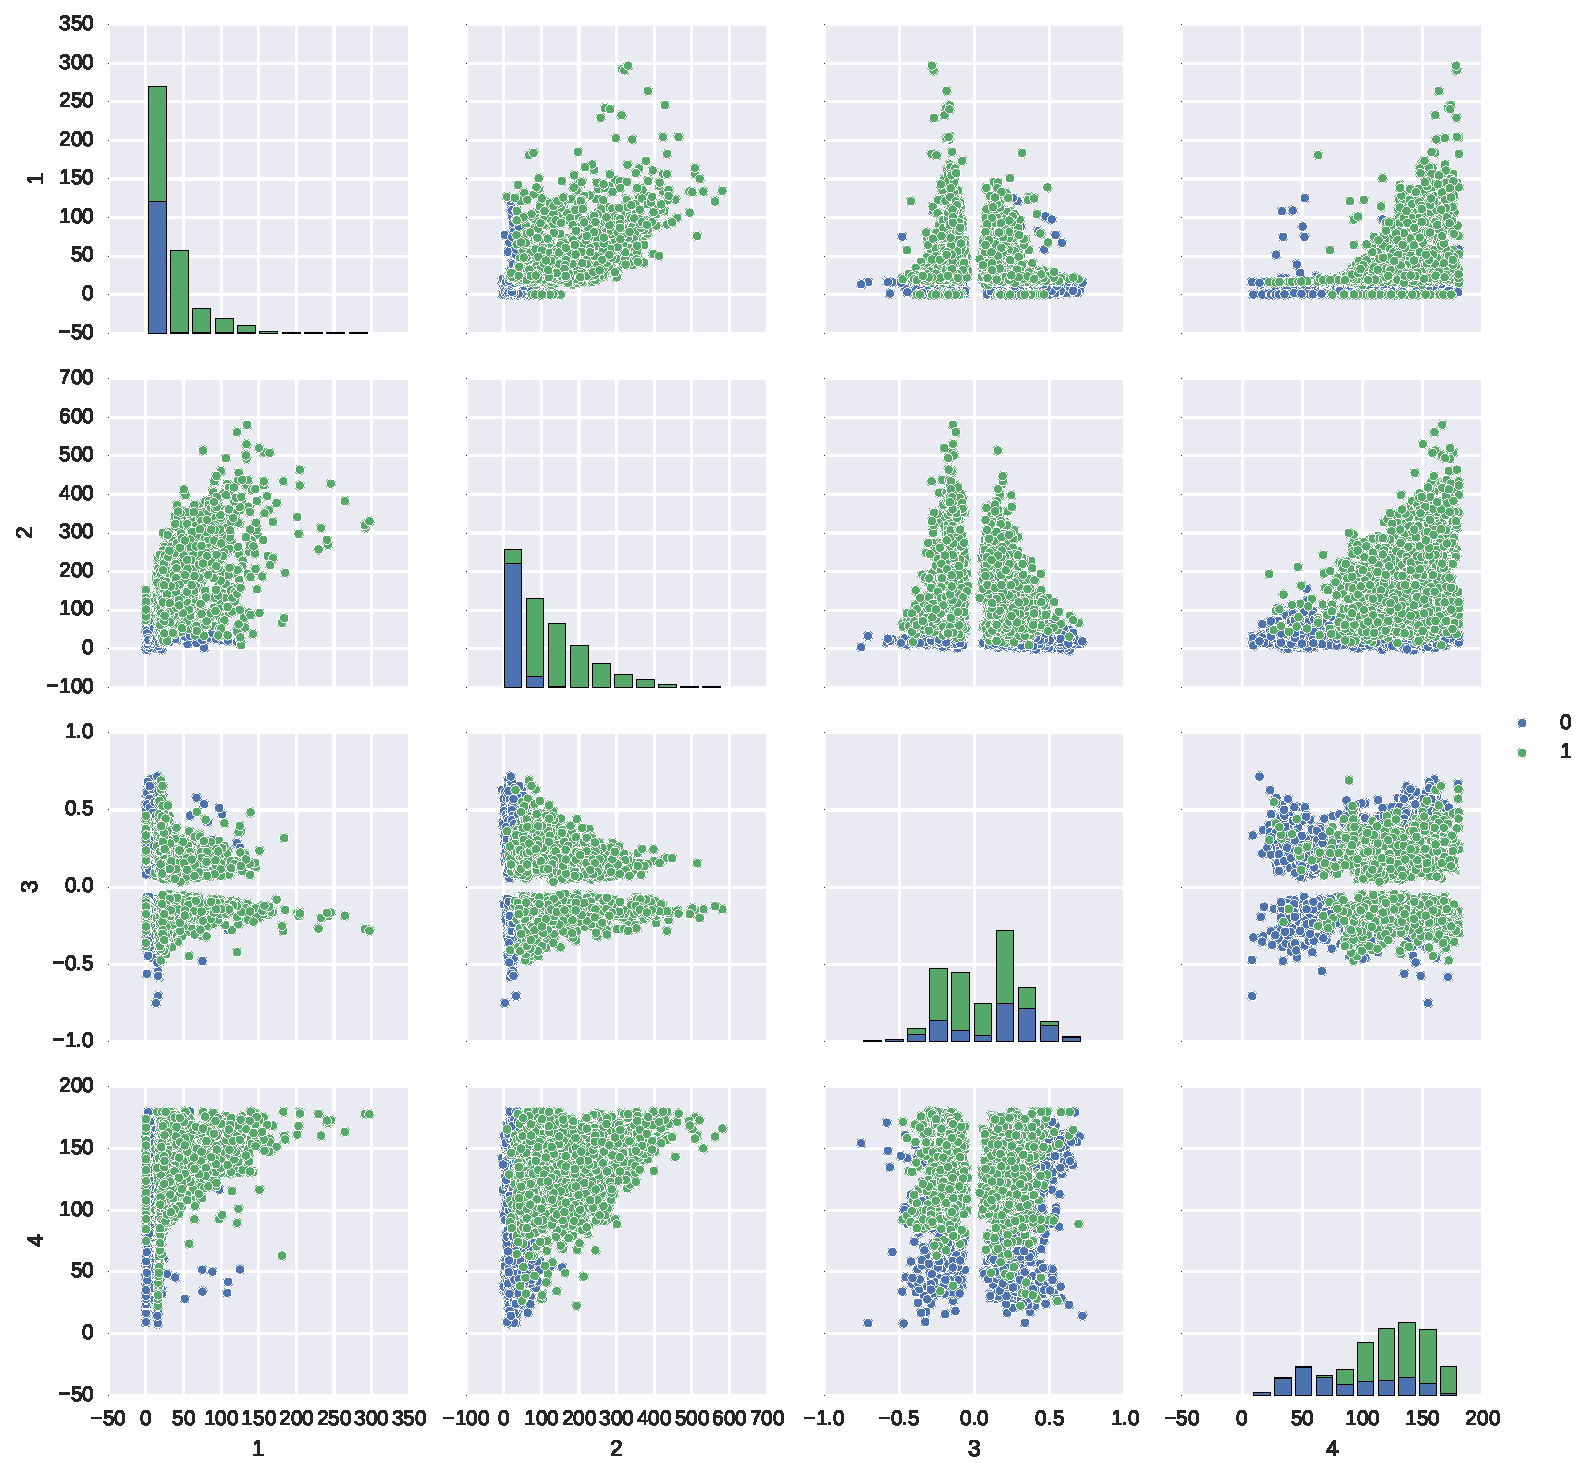
\includegraphics[width=0.8\textwidth]{figs/scatterplot.pdf}
  \caption{The scatterplot matrix of the dataset.}
  \label{fig:scatterplot}
\end{figure}

\section{Algorithm Design}
In order to train and test our classifier, firstly we set aside $\%25$ of the
observation as a testing set. The parameters of our classifiers are tuned
using 10-fold cross-validation using the rest $\%75$ observations.
Prior to the training, the data is preprocessed so that each feature has zero
mean and unit variance.

Since the dimension of the input variables is rather low and the number of
observations is relatively small, we first try to tune a simple
$k$-Nearest-Neighbor (KNN) classifier on the 4 given features. The results are
shown in Fig.~\ref{fig:knn_tune}. The 10-fold cross validation suggests that
when $k\in[3, 30]$ the validation score is maximized, where the KNN classifier 
results in a decent test score of $\sim0.95$. We select $k=15$ for our KNN
classifier.

\begin{figure}[h]
  \centering
  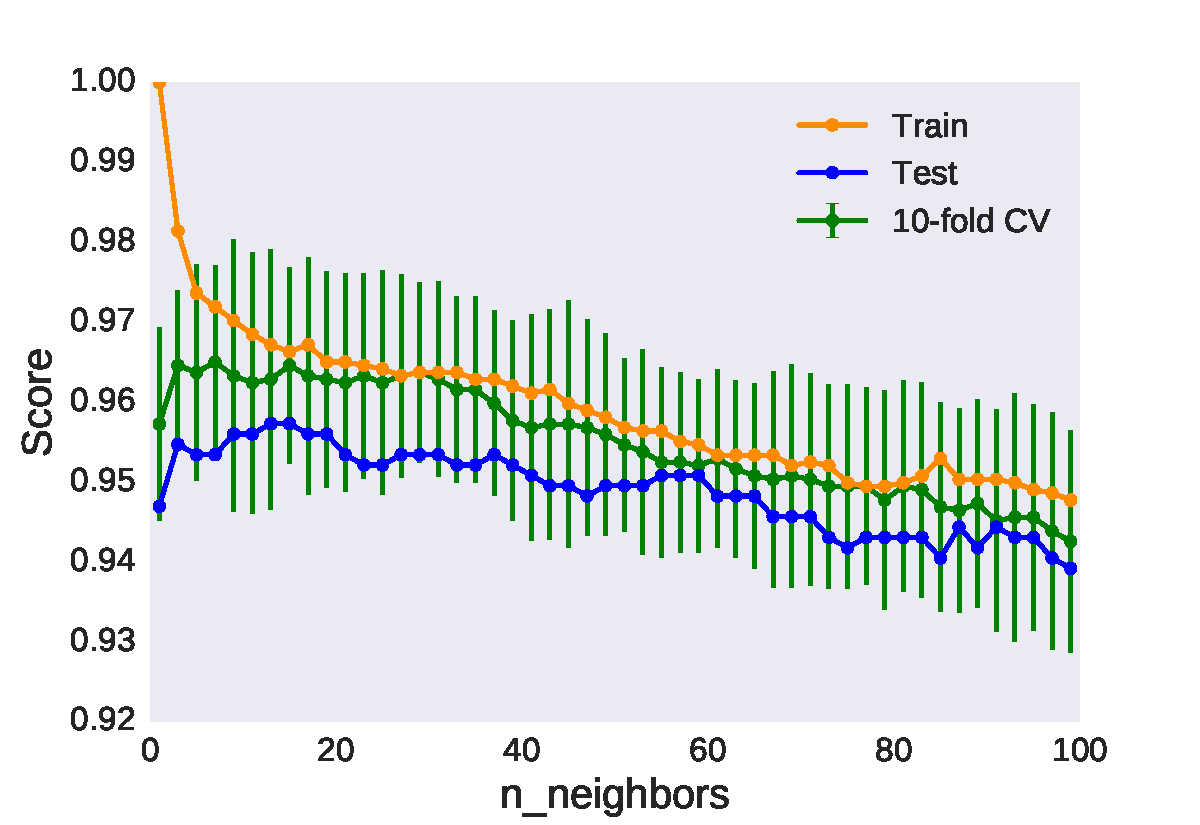
\includegraphics[width=0.5\textwidth]{figs/knn_tuning.pdf}
  \caption{Tuning the KNN classifier.}
  \label{fig:knn_tune}
\end{figure}

Although KNN results in a decent performance accuracy, we would like to try
other machine learning methods with better interpretability. Here we tried
decision tree model in which the depth of the tree is tuned with
cross-validation. The results is shown in Fig.~\ref{fig:tree_tune}. It appears
that the cross-validation favors a depth of 3 which also results in a test score
of $\sim0.95$, for which the decision tree fitted on the training set is shown
in Fig.~\ref{fig:tree_structure}.

\begin{figure}[h]
  \centering
  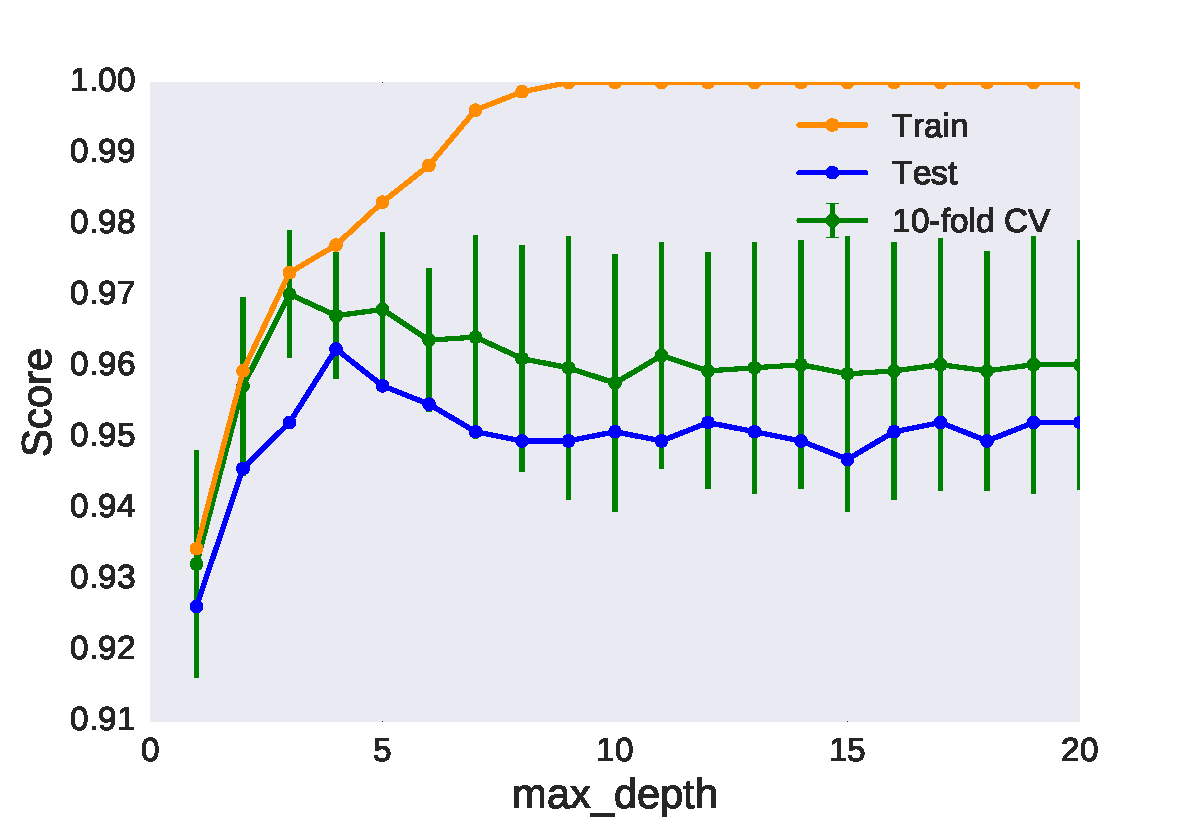
\includegraphics[width=0.5\textwidth]{figs/tree_tuning.pdf}
  \caption{Tuning the decision tree classifier.}
  \label{fig:tree_tune}
\end{figure}

\begin{figure}[h]
  \centering
  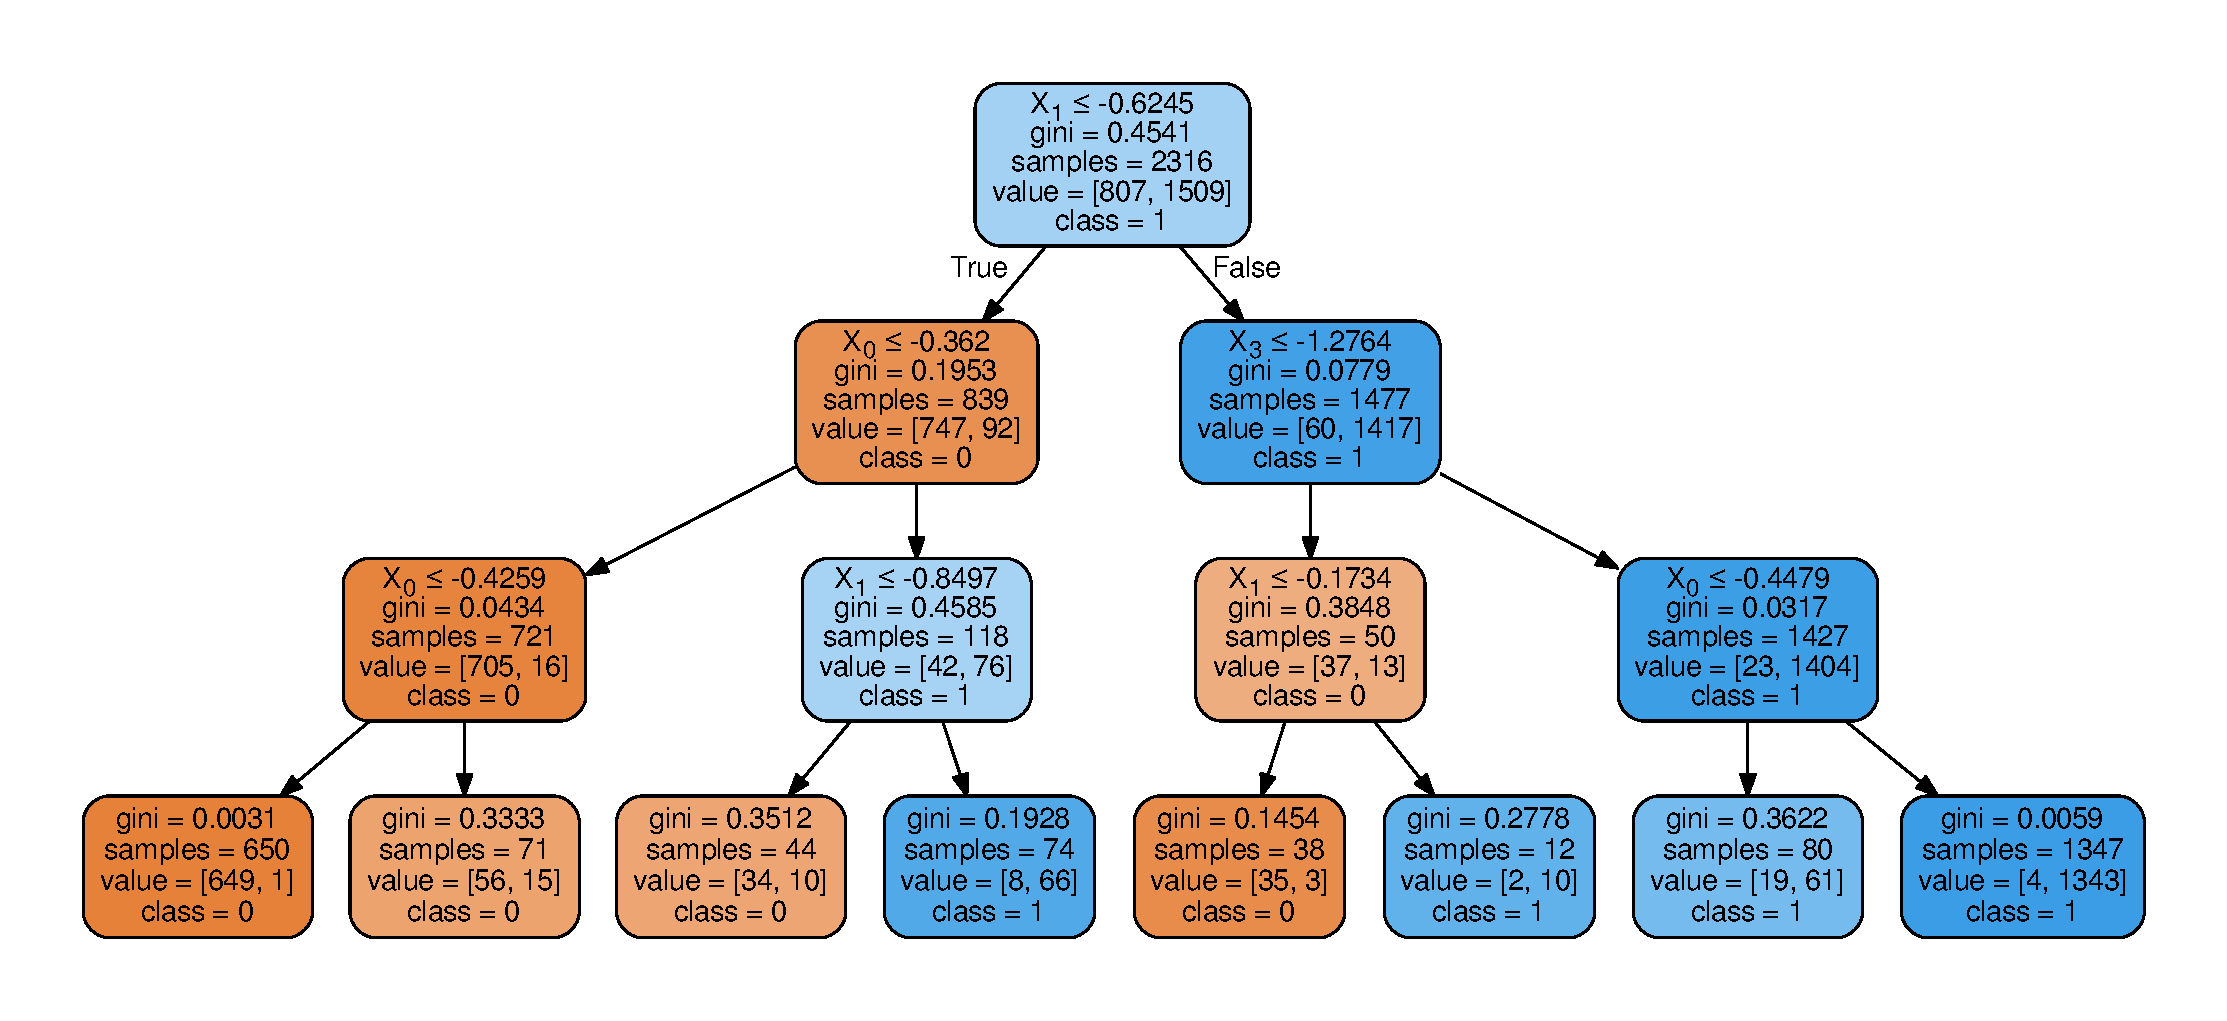
\includegraphics[width=0.9\textwidth]{figs/tree_structure.pdf}
  \caption{The trained decision tree classifier.}
  \label{fig:tree_structure}
\end{figure}

Nest we try some more rigorous (mathematically) machine learning techniques.
Firslty a discriminative model. Specifically, we applied the
logistic-regression method where the regularization parameter $C$ is chosen with
CV. The results are shown in Fig.~\ref{fig:logreg_tune}. It appears that
logistic regression does not work as good as other classifiers with a test score
of 0.944 for $C=1$.

\begin{figure}[h]
  \centering
  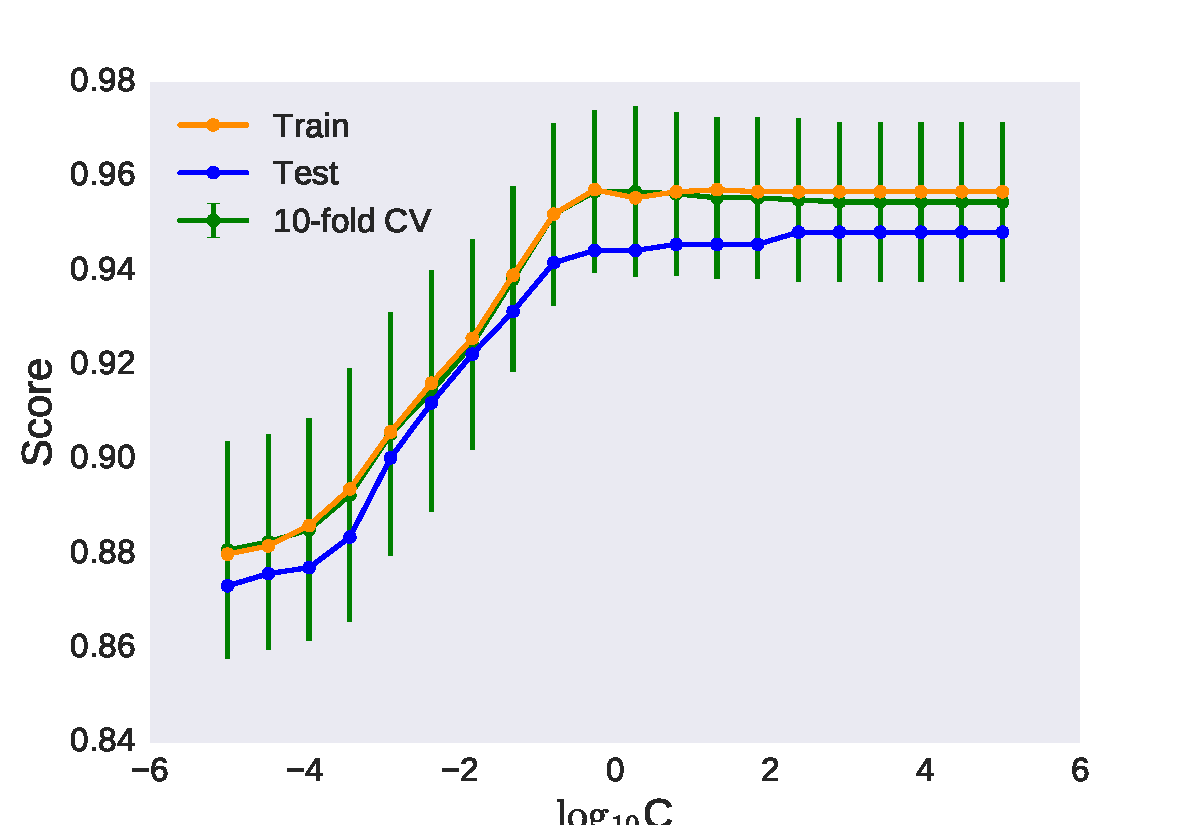
\includegraphics[width=0.7\textwidth]{figs/logreg_tuning.pdf}
  \caption{Tuning the logistic regression classifier.}
  \label{fig:logreg_tune}
\end{figure}

We would also like to see whether the performance can be improved with kernel
techniques and that promotes sparsities. We try to tune a SVM classifier with rbf kernel,
in which both the regularization parameter $C$ and the kernel parameter $\gamma$
are chosen with CV. The results are shown in Fig.~\ref{fig:svc_tune}. The SVC
achieve a tiny-slightly better test score of $0.96$ which should not be
considered as a significant performance gain. We select $C=1$ and $\gamma=1$ for
our SVM classifier.

\begin{figure}[h]
  \centering
  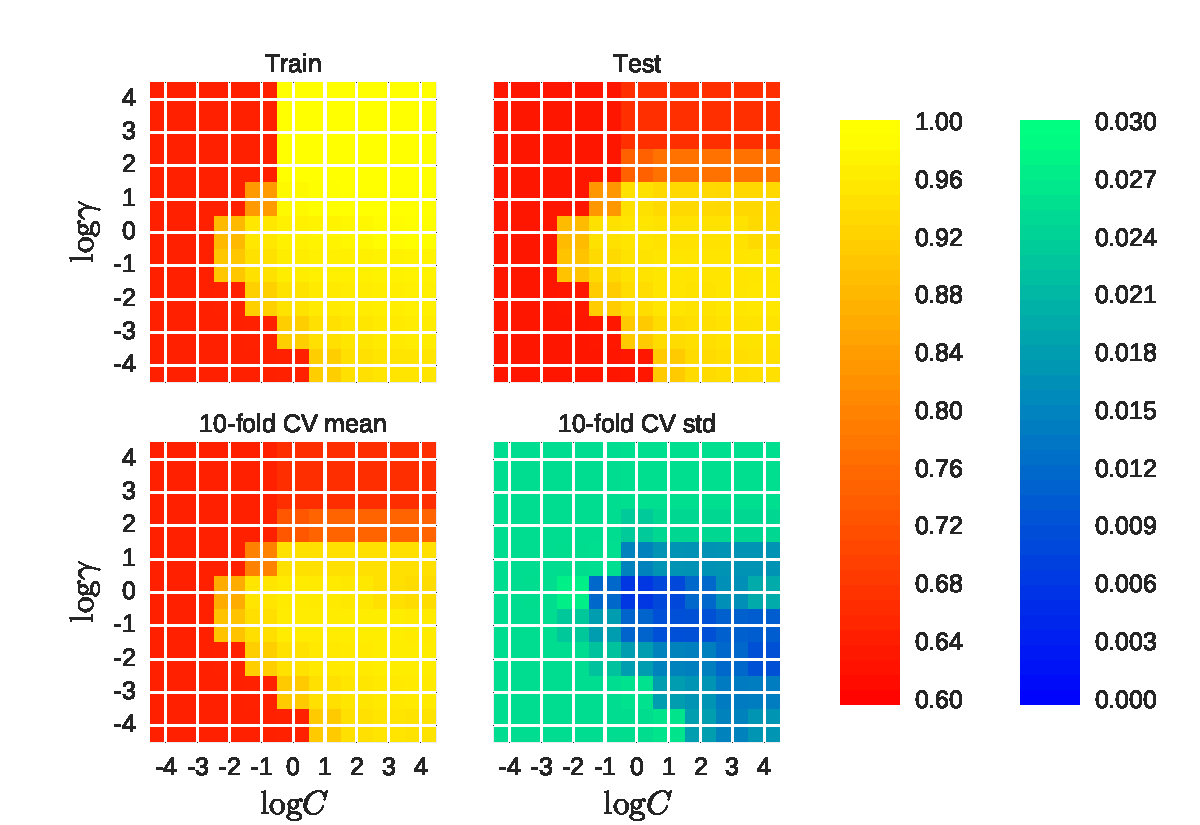
\includegraphics[width=0.7\textwidth]{figs/svc_tuning.pdf}
  \caption{Tuning the SVM classifier.}
  \label{fig:svc_tune}
\end{figure}

The classifiers we have tried so far are tuned with cross-validation, and as we
can see the choice of a single best classifier is usually unclear. To reduce the
variance of our classifier, we also tried the ensemble learning technique of
random forest. We fix the \texttt{max\_depth}=3 and trained a random forest of
10 trees. The resulting test score is $0.968$ which turns out to be a little
higher than the other classifiers.

As opposed to the frequentist approaches mentioned above, an arguably more
insightful and principled way of regularization is the Bayesian
approach.
In this study, we also tried two Bayesian classifiers, namely the relevance
vector machine (RVM) and the variational logistic
regression (VLR) implemented by Amazasp Shaumyan. For the RVM
classifier, we adopt the rbf kernel with $\gamma=1$. The RVM and VLR achieve
test scores of 0.961 and 0.944, respectively, which is almost the same as their
non-Bayesian counterparts.

\section{Numerical Results and Conclusion}
The performance of all the classifiers mentioned in the last section are
summarized in Table~\ref{table:comparison}. We decide to use the random forest
of 10 trees with max depth of 3 as our final classifier. A score of around 0.96
is expected from this classifier.

\begin{table}[!t]
  \renewcommand{\arraystretch}{1.3}
  \caption{Test performances of different classifiers.}
  \label{table:comparison}
  \centering
  \begin{tabular}{c|ccccc}
    \hline
    Classifier & false positive & false negative & precision & reall & score
    \\
    \hline
    KNN & 0.06383 & 0.03055 & 0.9382 & 0.9695 & 0.9573 \\
    Decision Tree & 0.08511 &  0.02648 & 0.9196 & 0.9735 & 0.9521 \\
    Log-Reg & 0.06738 & 0.04888 & 0.9338 & 0.9511 & 0.9444 \\
    SVM & 0.05674 & 0.03055 & 0.9447 & 0.9695 & 0.9599 \\
    Random Forest & 0.05674 & 0.02444 & 0.9450 & 0.9756 & 0.9638 \\
    RVM & 0.06738 & 0.02851 & 0.9351 & 0.9715 & 0.9573 \\
    Variational Log-Reg & 0.06738 & 0.04888 & 0.9338 & 0.9511 & 0.9444 \\
    \hline
  \end{tabular}
\end{table}

%   BIBLIOGRAPHY
%----------------------------------------------------------------------------------------

%\bibliographystyle{unsrt}
%\bibliography{myrefs}

%\pagebreak


%----------------------------------------------------------------------------------------


\end{document}